%%%%%%%%%%%%%%%%%%%%%%%%%%%%%%%%%%%%%
%                                   %
% Compile with XeLaTeX and biber    %
%                                   %
% Questions or comments:            %
%                                   %
% joshua dot mcneill at uga dot edu %
%                                   %
%%%%%%%%%%%%%%%%%%%%%%%%%%%%%%%%%%%%%

\documentclass{beamer}
  % Read in standard preamble (cosmetic stuff)
  %%%%%%%%%%%%%%%%%%%%%%%%%%%%%%%%%%%%%%%%%%%%%%%%%%%%%%%%%%%%%%%%
% This is a standard preamble used in for all slide documents. %
% It basically contains cosmetic settings.                     %
%                                                              %
% Joshua McNeill                                               %
% joshua dot mcneill at uga dot edu                            %
%%%%%%%%%%%%%%%%%%%%%%%%%%%%%%%%%%%%%%%%%%%%%%%%%%%%%%%%%%%%%%%%

% Beamer settings
% \usetheme{Berkeley}
\usetheme{CambridgeUS}
% \usecolortheme{dove}
% \usecolortheme{rose}
\usecolortheme{seagull}
\usefonttheme{professionalfonts}
\usefonttheme{serif}
\setbeamertemplate{bibliography item}{}

% Packages and settings
\usepackage{fontspec}
  \setmainfont{Charis SIL}
\usepackage{hyperref}
  \hypersetup{colorlinks=true,
              allcolors=blue}
\usepackage{graphicx}
  \graphicspath{{../../figures/}}
\usepackage[normalem]{ulem}
\usepackage{enumerate}

% Document information
\author{M. McNeill}
\title[FREN2001]{Français 2001}
\institute{\url{joshua.mcneill@uga.edu}}
\date{}

%% Custom commands
% Lexical items
\newcommand{\lexi}[1]{\textit{#1}}
% Gloss
\newcommand{\gloss}[1]{`#1'}
\newcommand{\tinygloss}[1]{{\tiny`#1'}}
% Orthographic representations
\newcommand{\orth}[1]{$\langle$#1$\rangle$}
% Utterances (pragmatics)
\newcommand{\uttr}[1]{`#1'}
% Sentences (pragmatics)
\newcommand{\sent}[1]{\textit{#1}}
% Base dir for definitions
\newcommand{\defs}{../definitions}


  % Packages and settings

  % Document information
  \subtitle[\lexi{C'est} et \lexi{il est}]{\lexi{C'est} et \lexi{il est}}

\begin{document}
  % Read in the standard intro slides (title page and table of contents)
  \begin{frame}
    \titlepage
    \tiny{Office: % Basically a variable for office hours location
Gilbert 121\\
          Office hours: % Basically a variable for office hours
 lundi, mercredi, vendredi 10:10--11:10
}
  \end{frame}

  \begin{frame}{Identification}
    \begin{columns}
      \column{0.5\textwidth}
        {\scriptsize
        Quelles sont leurs professions et leurs nationalités?
        \begin{enumerate}
          \item Toni Morrison
          \uncover<2-> {$\to$ Elle est écrivaine. C'est une écrivaine américaine.}
          \item<3-> Marion Cotillard
          \uncover<4-> {$\to$ Elle est actrice. C'est une actrice française.}
          \item<5-> Florence Nightingale
          \uncover<6-> {$\to$ Elle est infirmière. C'est une infirmière anglaise.}
          \item<7-> Albert Camus
          \uncover<8-> {$\to$ Il est écrivain. C'est un écrivain algérien.}
          \item<9-> Alexander Graham Bell
          \uncover<10->{$\to$ Il est ingénieur. C'est un ingénieur écossais.}
          \item<11-> Frank Gehry
          \uncover<12->{$\to$ Il est architecte. C'est un architecte canadien.}
          \item<13-> Francisco Goya
          \uncover<14->{$\to$ Il est artiste. C'est un artiste espagnol.}
        \end{enumerate}
        }
      \column{0.5\textwidth}
        \begin{minipage}[c][0.6\textheight]{\linewidth}
          \begin{center}
            \only<1-2>{
              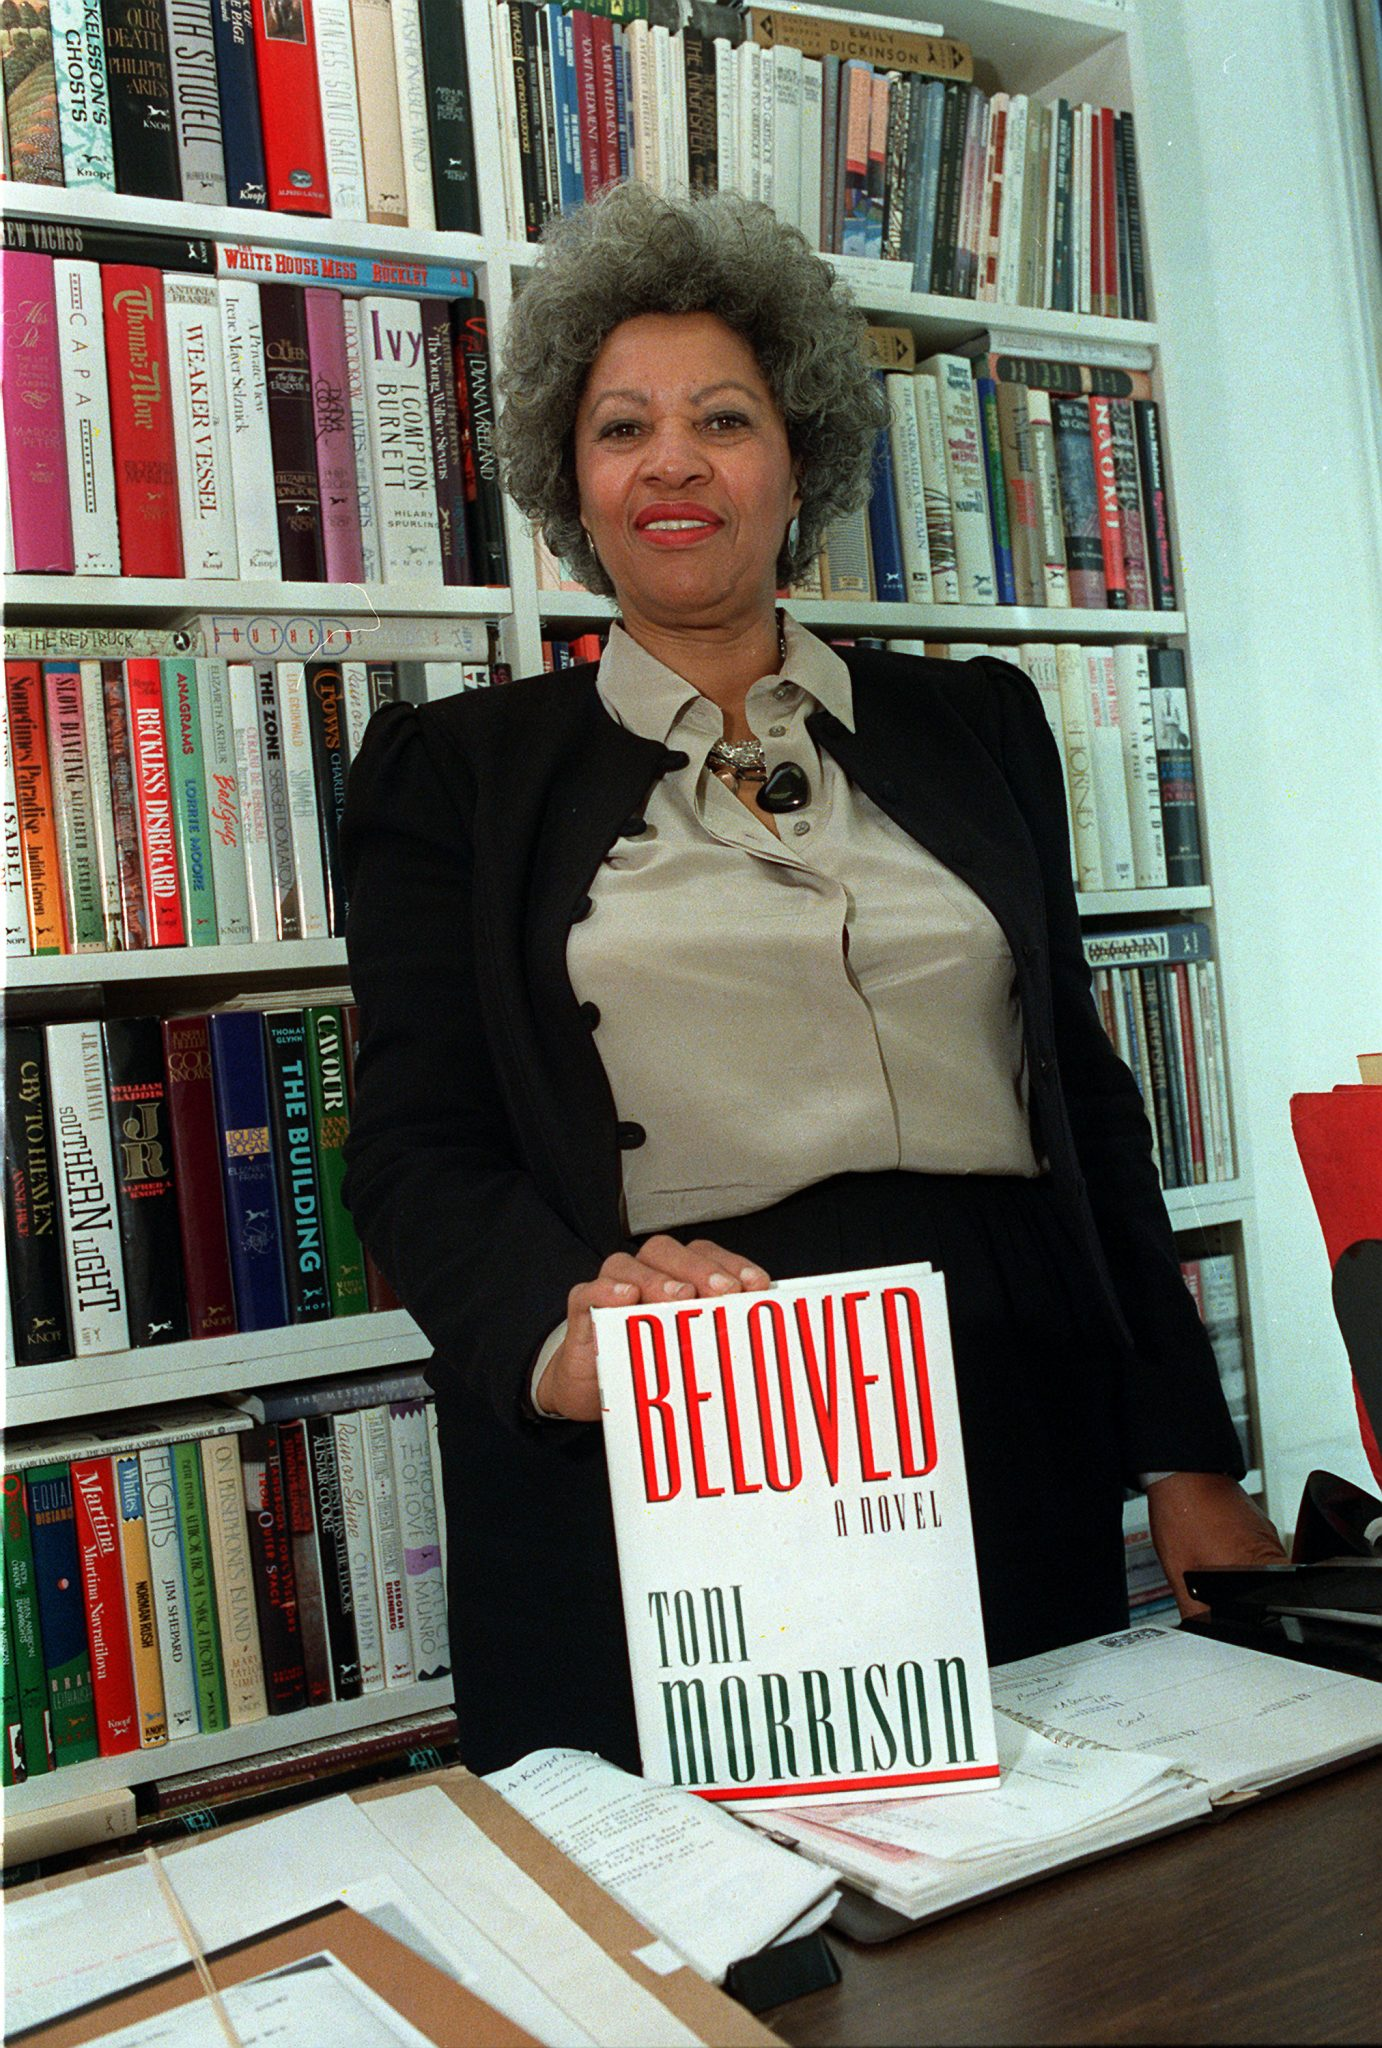
\includegraphics[scale=0.125]{toni_morrison.jpg}
            }
            \only<3-4>{
              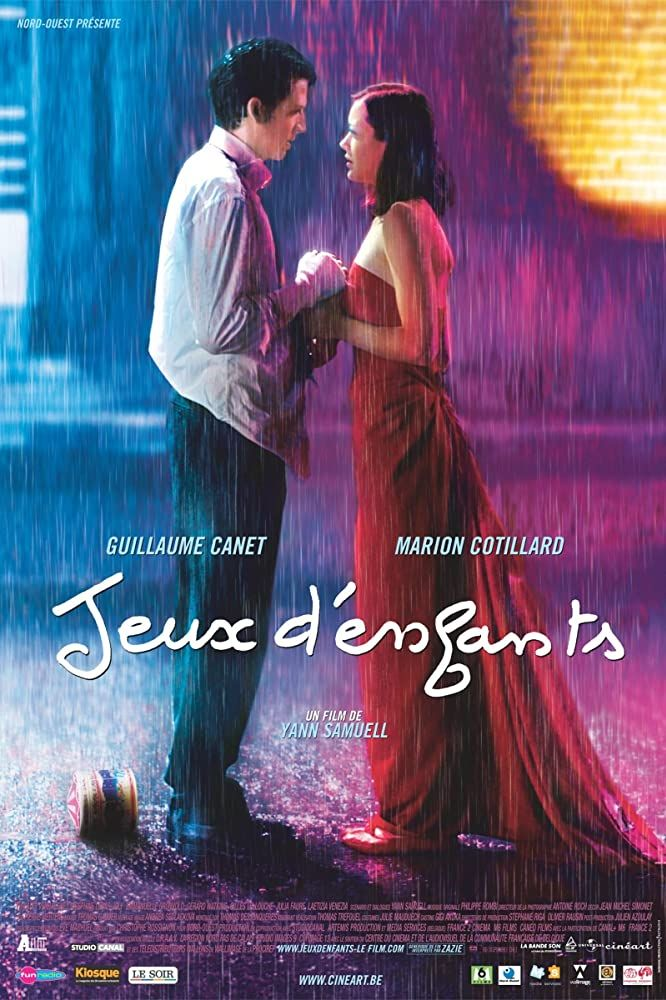
\includegraphics[scale=0.2]{marion_cotillard.jpg}
            }
            \only<5-6>{
              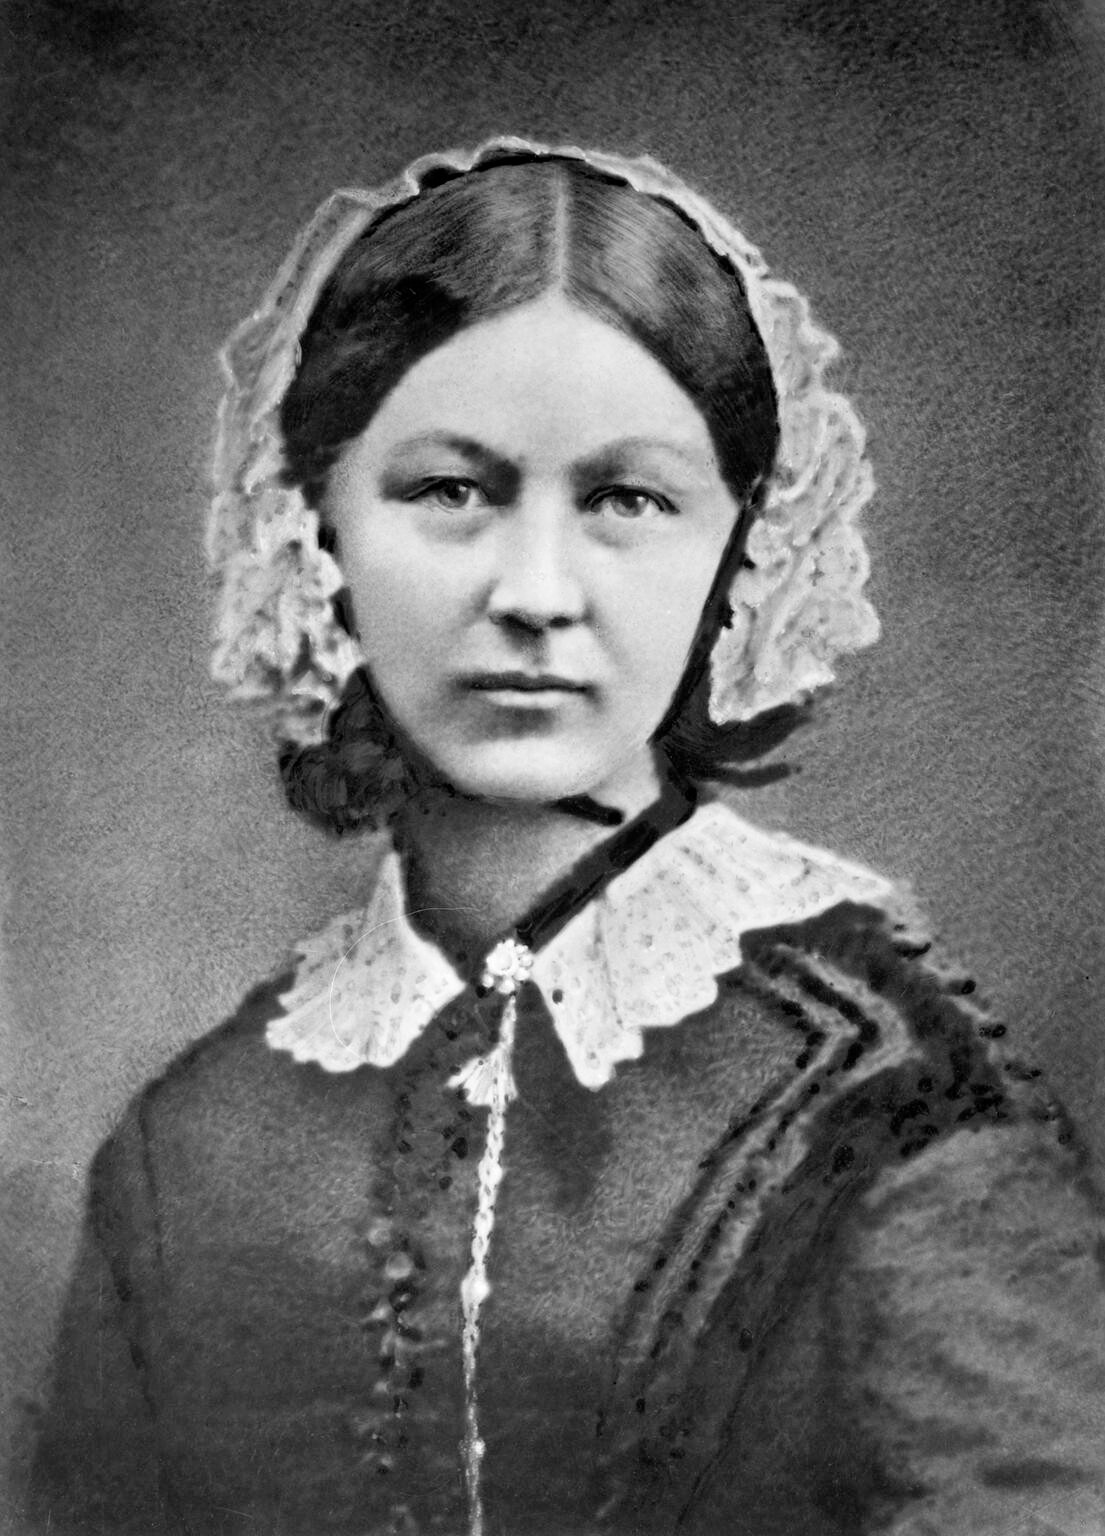
\includegraphics[scale=0.5]{florence_nightingale.jpg}
            }
            \only<7-8>{
              
\includegraphics[scale=0.3]{albert_camus.png}
            }
            \only<9-10>{
              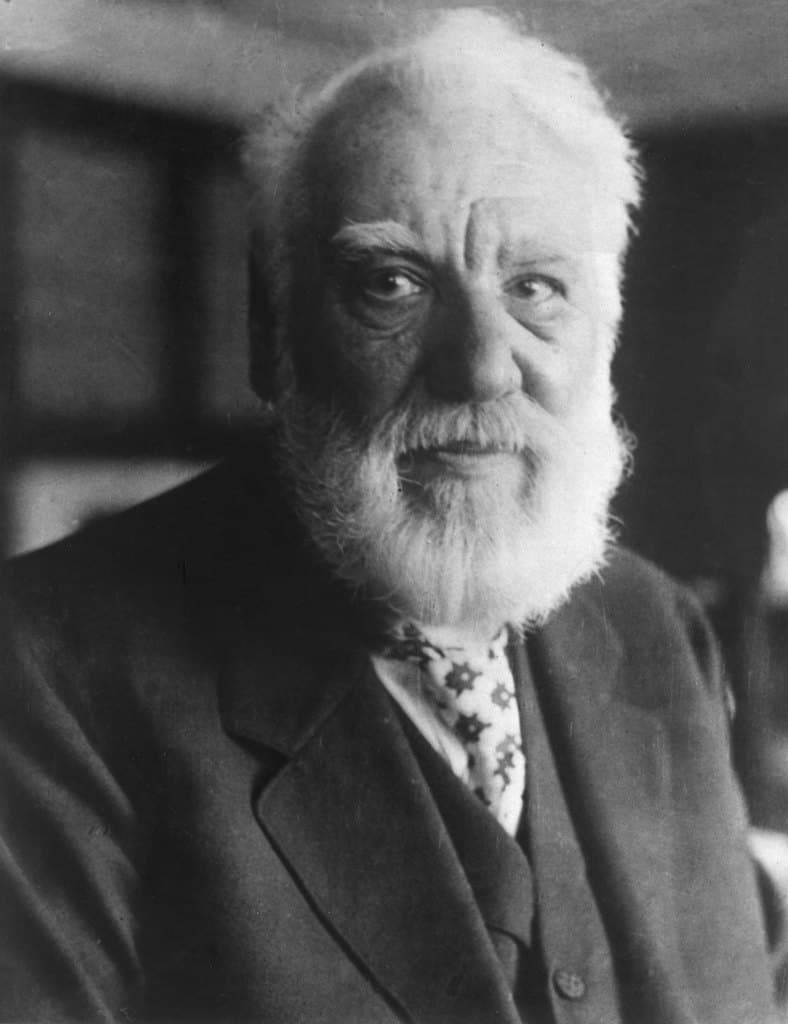
\includegraphics[scale=0.18]{alexander_bell.jpg}
            }
            \only<11-12>{
              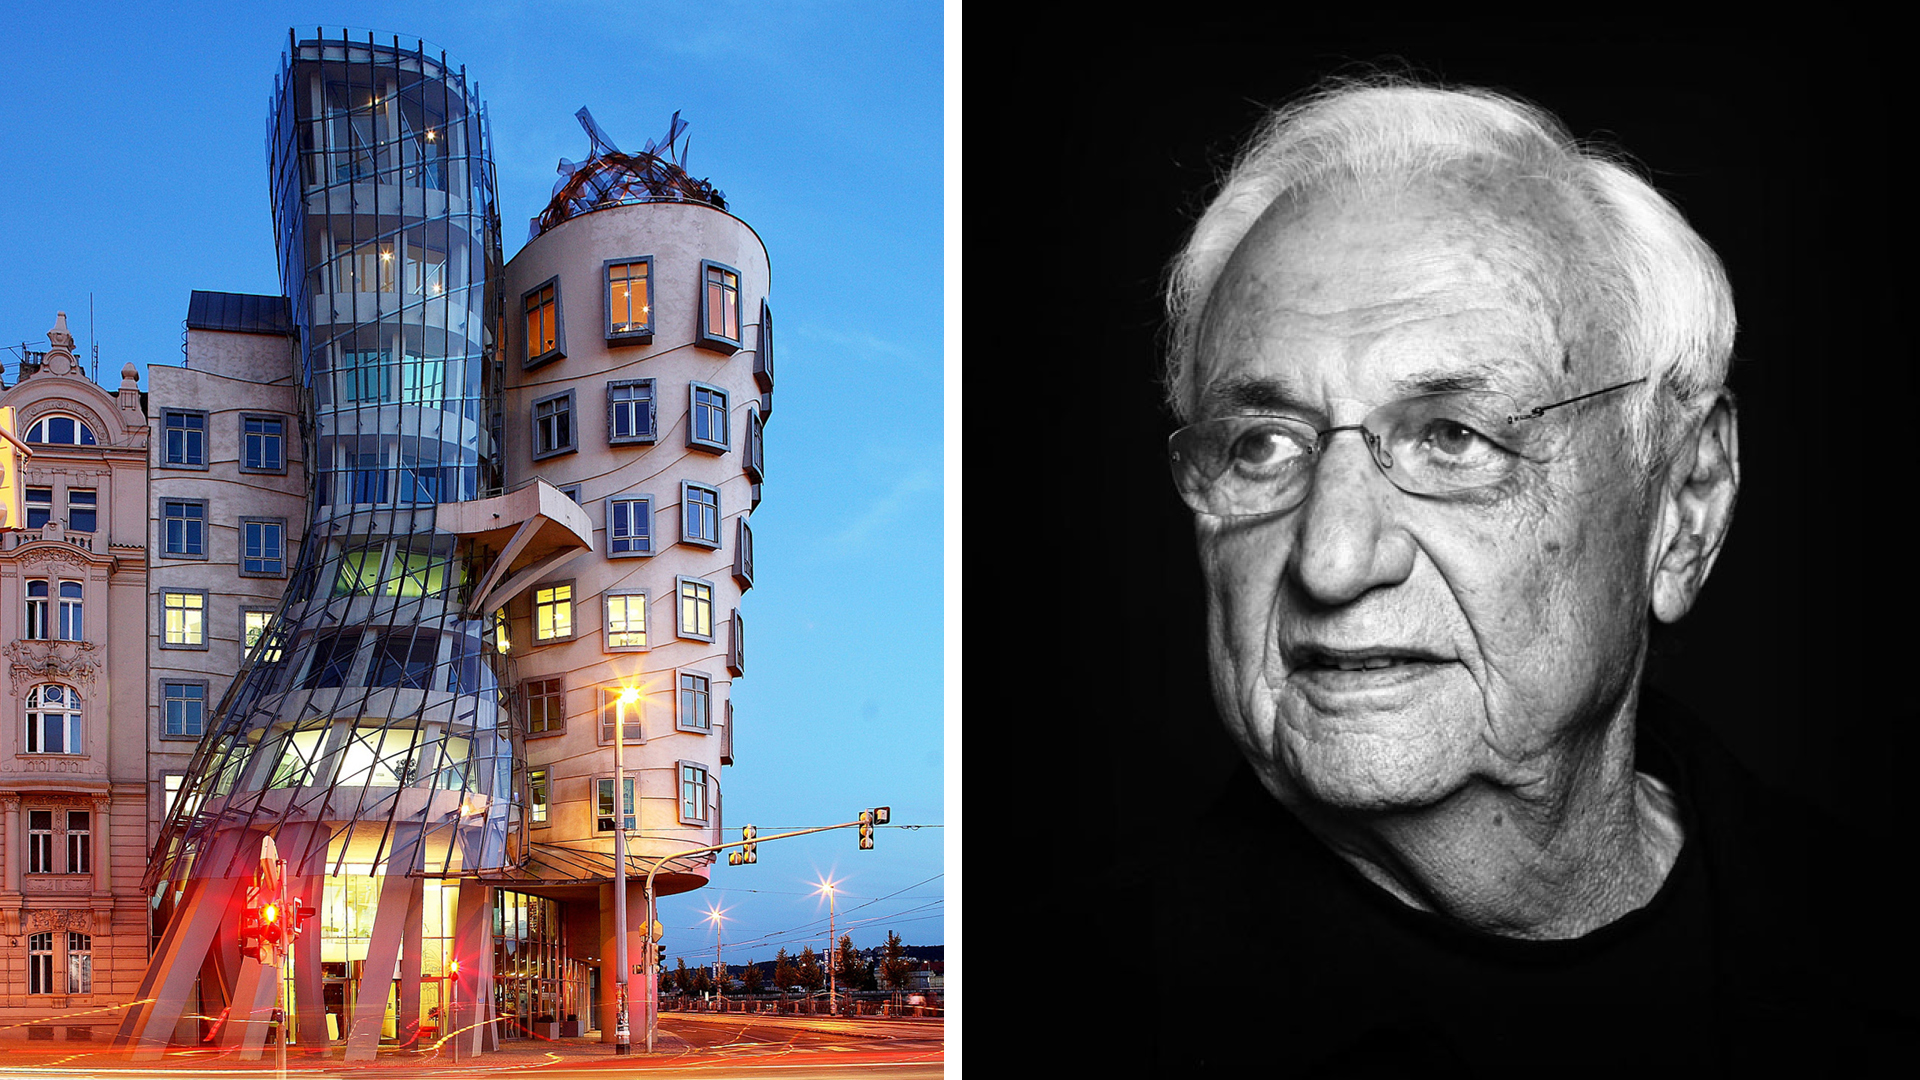
\includegraphics[scale=0.085]{frank_gehry.jpg}
            }
            \only<13-14>{
              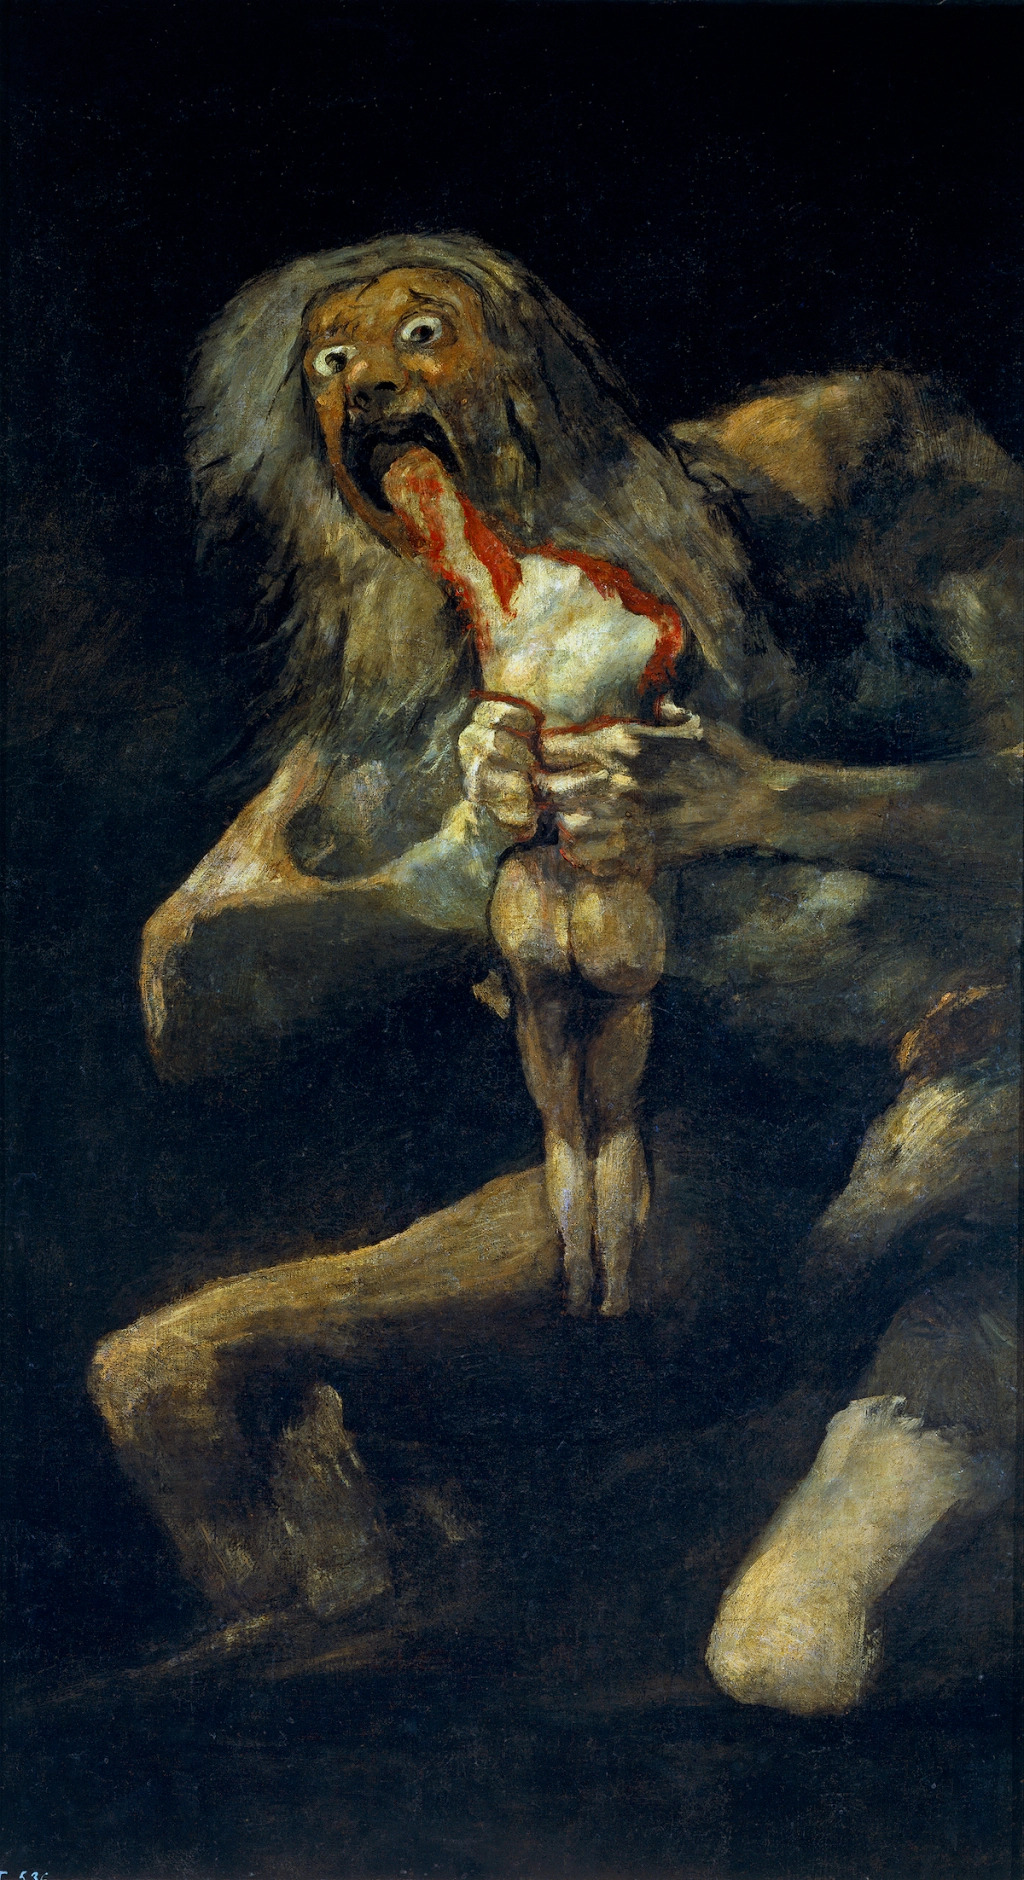
\includegraphics[scale=0.095]{goya.jpg} \\
              Saturno devorando a su hijo (1819-1823)
            }
          \end{center}
        \end{minipage}
    \end{columns}
  \end{frame}

  \begin{frame}{}
    \begin{center}
      \Large Quiz
    \end{center}
  \end{frame}

  \begin{frame}{Qu'est-ce que je fais?}
    En groupes de 3 ou 4, mets une carte avec une profession sur ton front chacun à son tour, et essaie de deviner la profession à partir des descriptions de la profession que tes camarades de groupe te donnent. \\
    \tinygloss{In groups of 3 or 4, take turns placing a card  with a profession on your forehead, and try to guess the profession from the descriptions of the profession that your groupmates give you.}
    \begin{columns}
      \column{0.6\textwidth}
        \begin{description}
          \item[] \textbf{Modèle:}
          \item[] \emph{docteur/e} (on E1's forehead)
          \item[E2:] Tu adores aider les personnes à l'hôpital.
          \item[E3:] Tu as un gros salaire.
          \item[E1:] Je suis docteur/e?
        \end{description}
        \begin{center}
          \scriptsize
          \textbf{Useful vocab on page 127 of your textbook.}
        \end{center}
      \column{0.4\textwidth}
        \begin{center}
          
\includegraphics[scale=0.5]{headsup.jpg}
        \end{center}
    \end{columns}
  \end{frame}

  \begin{frame}{Quelle est sa profession?}
    Dis à ton/ta partenaire ce que les personnes dans ta famille suivantes font comme métier. \\
    \tinygloss{Tell your partner what the following people in your family do.}
    \begin{columns}
      \column{0.5\textwidth}
        \begin{description}
          \item[] \textbf{Modèle:}
          \item[] \emph{ta mère}
          \item[E1:] Ma mère est assistante sociale.
          \item[E2:] C'est une bonne avocate, ma mère.
        \end{description}
      \column{0.5\textwidth}
        \begin{enumerate}
          \item ta mère
          \item ton père
          \item ton frère ou ta sœur
          \item ton oncle ou ta tante
          \item ton grand-père ou ta grand-mère
        \end{enumerate}
    \end{columns}
  \end{frame}

  \begin{frame}{}
    \begin{center}
      \Large Questions?
    \end{center}
  \end{frame}
\end{document}
